\documentclass[xetex,mathserif,serif]{beamer}
\usepackage{polyglossia}
\setdefaultlanguage[babelshorthands=true]{russian}
\usepackage{minted}
\usepackage{tabu}

\useoutertheme{infolines}

\usepackage{fontspec}
\setmainfont{FreeSans}
\newfontfamily{\russianfonttt}{FreeSans}

\setbeamertemplate{blocks}[rounded][shadow=false]
\setbeamercolor*{block title example}{fg=green!50!black,bg=green!20}
\setbeamercolor*{block body example}{fg=black,bg=green!10}

\setbeamercolor*{block title alerted}{fg=red!50!black,bg=red!20}
\setbeamercolor*{block body alerted}{fg=black,bg=red!10}

\tabulinesep=0.7mm

\title{Проектирование пользовательских интерфейсов}
\author[Юрий Литвинов]{Юрий Литвинов \newline \textcolor{gray}{\small\texttt{yurii.litvinov@gmail.com}}}

\date{16.03.2018г}

\begin{document}
	
	\frame{\titlepage}

	% \section{Разбор CLI}

	% \begin{frame}
	% 	\frametitle{Комментарии по домашней работе}
	% 	\begin{itemize}
	% 		\item Исправления надо тоже отмечать на HwProj (ссылкой на тот же пуллреквест)
	% 		\item ``Каноничное'' именование пакетов в Java --- ru.spbau.mit....
	% 		\begin{itemize}
	% 			\item Не в Java всё равно лучше завести корневой пакет/неймспейс для проекта
	% 		\end{itemize}
	% 		\item try/catch в тестах не по делу
	% 		\begin{itemize}
	% 			\item \mintinline{java}|@Test(expected=NullReferenceException.class)|
	% 		\end{itemize}
	% 		\item Говорящие имена тестов, например, ShouldNotCrashWhenNoArgsTest
	% 		\item Синглтоны следует применять с осторожностью
	% 		\item Принимать параметры и возвращать значения лучше как интерфейсы, а не как конкретные классы
	% 		\item Реализации команд --- методы одного класса или отдельные классы?
	% 	\end{itemize}
	% \end{frame}

	% \begin{frame}
	% 	\frametitle{Архитектура типового <<хорошего>> решения}
	% 	\begin{center}
	% 		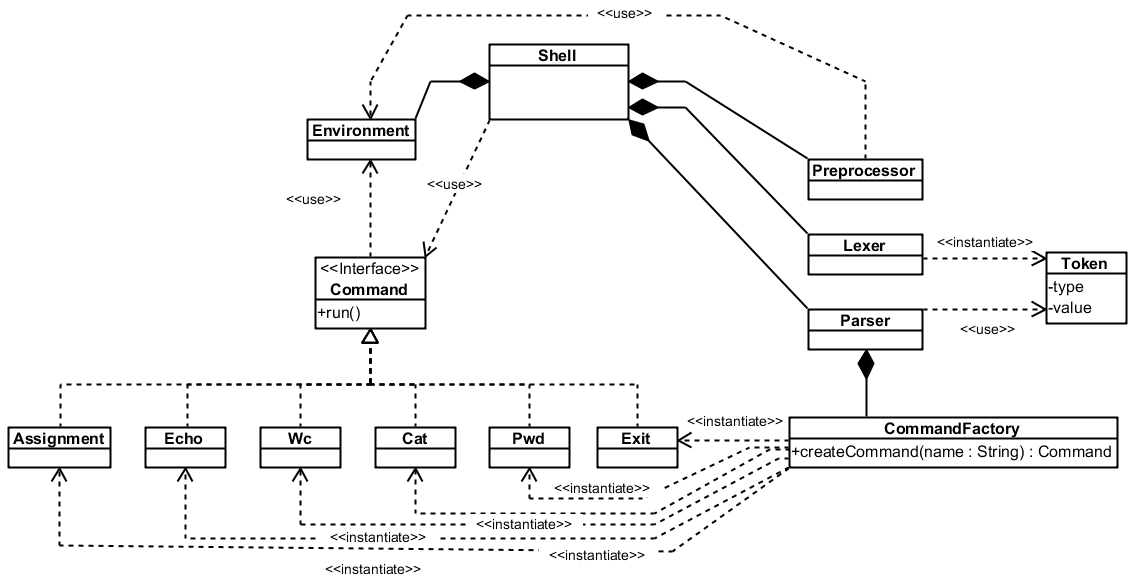
\includegraphics[width=\textwidth]{cliArchitecture.png}
	% 	\end{center}
	% \end{frame}

	\section{Проектирование пользовательских интерфейсов}

	\begin{frame}
		\frametitle{Screen flow}
		\begin{columns}
			\begin{column}{0.6\textwidth}
				\begin{itemize}
					\item Показывает возможные переходы между страницами
					\item Проектируется исходя из пользовательских сценариев
					\item Полезен как ``обзор'' приложения
				\end{itemize}
			\end{column}
			\begin{column}{0.4\textwidth}
				\begin{center}
					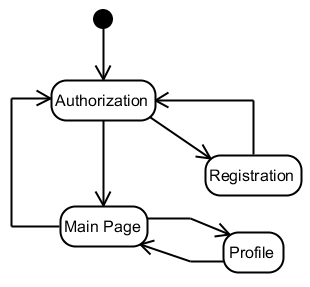
\includegraphics[width=0.8\textwidth]{screenFlow.png}
				\end{center}
			\end{column}
		\end{columns}
	\end{frame}

	\begin{frame}
		\frametitle{Wireframe}
		\begin{columns}
			\begin{column}{0.4\textwidth}
				\begin{itemize}
					\item Набор схематичных макетов
					\item Принципиально без дизайнерских подробностей, только положение элементов
					\item Используется как ТЗ, наглядный материал, первое приближение к дизайну
				\end{itemize}
			\end{column}
			\begin{column}{0.6\textwidth}
				\begin{center}
					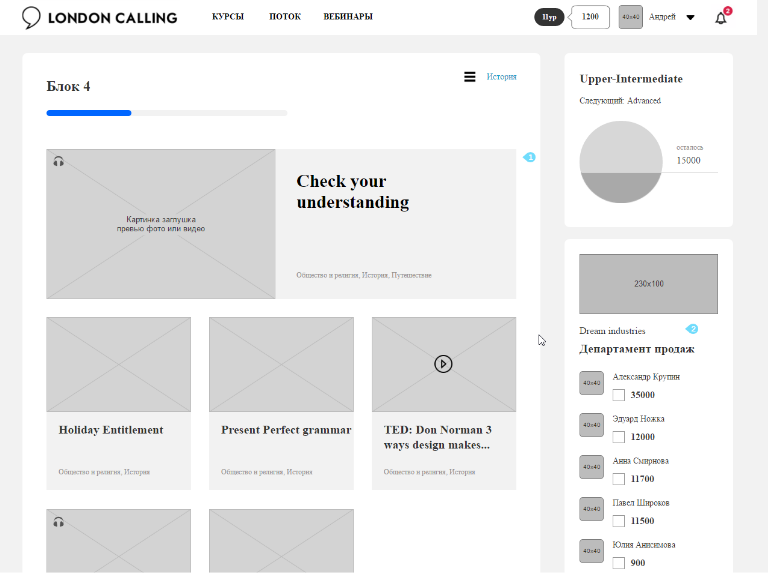
\includegraphics[width=\textwidth]{wireframe.png}
				\end{center}
			\end{column}
		\end{columns}
	\end{frame}

	\begin{frame}
		\frametitle{Дизайн-макет}
		\begin{columns}
			\begin{column}{0.4\textwidth}
				\begin{itemize}
					\item Разрабатывается дизайнером
					\item Похож на окончательный внешний вид интерфейса
					\item Часто с точностью до пиксела
				\end{itemize}
			\end{column}
			\begin{column}{0.6\textwidth}
				\begin{center}
					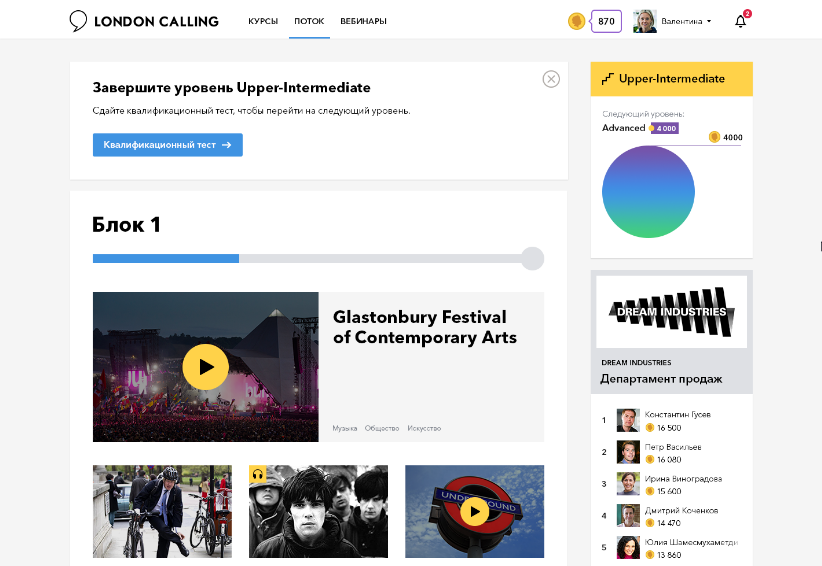
\includegraphics[width=\textwidth]{mockup.png}
				\end{center}
			\end{column}
		\end{columns}
	\end{frame}

	\begin{frame}
		\frametitle{Инструменты проектирования пользовательских интерфейсов}
		\begin{itemize}
			\item Balsamiq
			\begin{itemize}
				\item \url{https://balsamiq.com/products/mockups/}
				\item Кликабельные .pdf-ки
			\end{itemize}
			\item Ninjamock
			\begin{itemize}
				\item \url{https://ninjamock.com/}
				\item Бесплатный
				\item Веб-версия с коллаборацией
			\end{itemize}
			\item Axure
			\begin{itemize}
				\item \url{http://www.axure.com/}
				\item Продвинутый, но платный
			\end{itemize}
			\item UXPin
			\begin{itemize}
				\item \url{https://www.uxpin.com/}
				\item Продвинутый, но платный
				\item Зато браузерный
			\end{itemize}
		\end{itemize}
	\end{frame}

	\begin{frame}
		\frametitle{Ещё инструменты}
		\begin{itemize}
			\item Sketch
			\begin{itemize}
				\item \url{https://www.sketchapp.com/}
				\item Только под Mac
				\item Рисовалка интерфейсов, иконок и прочего
			\end{itemize}
			\item Figma
			\begin{itemize}
				\item \url{https://www.figma.com}
				\item Браузерный, коллаборативный
			\end{itemize}
			\item Invision app
			\begin{itemize}
				\item \url{https://www.invisionapp.com/}
				\item Браузерный, коллаборативный
				\item Кликабельные мокапы из картинок или Sketch-файлов
			\end{itemize}
		\end{itemize}
	\end{frame}

	\begin{frame}
		\frametitle{Visual Paradigm}
		\url{https://www.visual-paradigm.com/download/community.jsp}
		\begin{itemize}
			\item Одна из самых популярных CASE-систем
			\item Нам потребуется для рисования UML-диаграмм
			\item В ней можно рисовать Screen Flow как диаграммы активностей
			\item Надо скачать и поставить к следующему занятию
		\end{itemize}
	\end{frame}

	\begin{frame}
		\frametitle{Задача, HwProj}
		Спроектировать интерфейс приложения HwProj таким, каким вы его видите в идеале (со стороны студента и пофантазировать на тему функциональности препода)
		\begin{itemize} 
			\item Исполнение --- на ваше усмотрение (мобильное, настольное или веб-приложение)
			\item Функциональность тоже может отличаться (например, можно добавить элементы игрофикации)
		\end{itemize} 
		Что нужно сделать:
		\begin{itemize} 
			\item Описать поток экранов HwProj в виде UML-диаграммы активностей
			\item Сделать набор макетов всех экранов приложения в каком-либо из инструментов создания wireframe-макетов 
		\end{itemize} 
		Результаты выложить на гитхаб и/или приаттачить ссылку на проект в каком-либо из онлайн-тулов
	\end{frame}

	\section{Библиотеки логирования}

	\begin{frame}
		\frametitle{Внезапно, логирование}
		\begin{itemize}
			\item Отладочный вывод --- дешёвая альтернатива отладке
			\begin{itemize}
				\item Иногда быстрее вставить отладочную печать, чем проходить отладчиком
				\item Иногда отладчик недоступен или бесполезен
				\begin{itemize}
					\item Многопоточные и распределённые приложения
					\item Встроенные системы
				\end{itemize}
			\end{itemize}
			\item Post-mortem-анализ
			\begin{itemize}
				\item ``Отладочный вывод'' должен работать и на развёрнутой системе
				\item И выводить не в консоль
				\item И обеспечивать информацию о контексте
			\end{itemize}
			\item Примерно 4\% кода типичных проектов связано с логированием
			\item Стратегическая расстановка операций логирования --- важная часть архитектуры
		\end{itemize}
	\end{frame}

	\begin{frame}
		\frametitle{Apache Log4j 2, основные понятия}
		\begin{description}
			\item [Logger] --- штука, которая может что-то куда-то выводить (на самом деле, производить логирующие события)
			\item [LoggerConfig] --- управляет поведением логгера
			\item [LogManager] --- создаёт, хранит и выдаёт по запросу логгеры
			\item [Filter] --- фильтрует логирующие события, говоря, надо или не надо их куда-то выводить
			\item [Appender] --- на самом деле выводит информацию куда-то (в файл, на консоль, в системный лог и т.д.)
			\item [Layout] --- говорит, в каком формате и какую информацию о событии следует выводить
		\end{description}
		\begin{center}Вся конфигурация --- иерархическая\end{center}
	\end{frame}

	\begin{frame}
		\frametitle{Архитектура}
		\begin{center}
			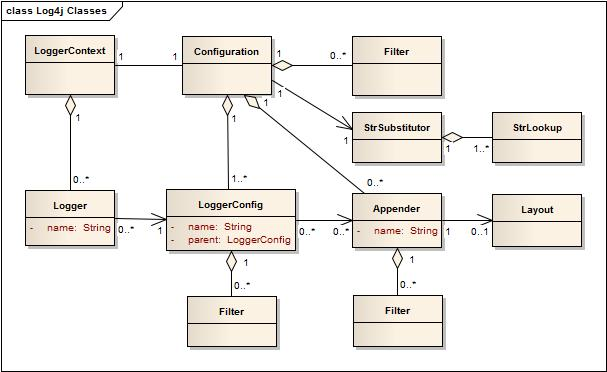
\includegraphics[width=0.8\textwidth]{log4jClasses.jpg}
		\end{center}
	\end{frame}

	\begin{frame}[fragile]
		\frametitle{Пример}
		\begin{minted}{java}
import org.apache.logging.log4j.LogManager;
import org.apache.logging.log4j.Logger;
 
public class HelloWorld {
    private static final Logger logger 
            = LogManager.getLogger("HelloWorld");
    public static void main(String[] args) {
        logger.info("Hello, World!");
    }
}
		\end{minted}
\end{frame}

	\begin{frame}[fragile]
		\frametitle{Пример конфигурации}
		\begin{minted}{xml}
<?xml version="1.0" encoding="UTF-8"?>
<Configuration monitorInterval="30">
  <Appenders>
    <Console name="Console" target="SYSTEM_OUT">
      <PatternLayout pattern=
          "%d{HH:mm:ss.SSS} [%t] %-5level %logger{36} - %msg%n"/>
    </Console>
  </Appenders>
  <Loggers>
    <Root level="error">
      <AppenderRef ref="Console"/>
    </Root>
  </Loggers>
</Configuration>
		\end{minted}
\end{frame}

	\begin{frame}
		\frametitle{Куда это писать}
		Log4j ищет конфигурации в следующих местах в следующем порядке:
		\begin{itemize}
			\item Системное свойство ``log4j.configurationFile'' (указывается при запуске опцией -D)
			\item log4j2-test.properties в classpath
			\item log4j2-test.yaml или log4j2-test.yml в classpath
			\item log4j2-test.json или log4j2-test.jsn в classpath
			\item log4j2-test.xml в classpath
			\item log4j2.properties в classpath
			\item log4j2.yaml или log4j2.yml в classpath
			\item log4j2.json или log4j2.jsn в classpath
			\item log4j2.xml в classpath
			\item Иначе используется DefaultConfiguration, которая выводит на консоль
		\end{itemize}
	\end{frame}

	\begin{frame}[fragile]
		\frametitle{Уровни и маркеры}
		Уровни логирования: \textbf{TRACE}, \textbf{DEBUG}, \textbf{INFO}, \textbf{WARN}, \textbf{ERROR}, \textbf{FATAL}, \textbf{OFF}

		Маркеры --- способ тонкой настройки информации, которую хочется выводить. Пример:
		\begin{minted}{java}
private static final Marker SQL_MARKER 
        = MarkerManager.getMarker("SQL");

private static final Marker QUERY_MARKER 
        = MarkerManager.getMarker("SQL_QUERY")
                       .setParents(SQL_MARKER);
...
logger.debug(QUERY_MARKER, "SELECT * FROM {}", table);
		\end{minted}
\end{frame}

	\begin{frame}[fragile]
		\frametitle{Синтаксис конфигурации (1)}
		\begin{minted}{xml}
<?xml version="1.0" encoding="UTF-8"?>
<Configuration>
  <Properties>
    <Property name="name1">value</property>
    <Property name="name2" value="value2"/>
  </Properties>
  <Filter type="type" ... />
  <Appenders>
    <Appender type="type" name="name">
      <Filter type="type" ... />
    </Appender>
    ...
  </Appenders>
		\end{minted}
\end{frame}

	\begin{frame}[fragile]
		\frametitle{Синтаксис конфигурации (2)}
		\begin{minted}{xml}
  <Loggers>
    <Logger name="name1">
      <Filter type="type" ... />
    </Logger>
    ...
    <Root level="level">
      <AppenderRef ref="name"/>
    </Root>
  </Loggers>
</Configuration>
		\end{minted}
\end{frame}

	\begin{frame}
		\frametitle{Appenders}
		\begin{description}
			\item [Console] --- выводит в SYSTEM\_OUT или SYSTEM\_ERR
			\item [File] --- выводит в указанный файл
			\item [RollingFile] --- выводит в указанный файл, создавая новые файлы и удаляя старые при необходимости
			\begin{itemize}
				\item TriggeringPolicy --- когда переходить к следующему файлу и что-то делать с предыдущими
				\begin{itemize}
					\item При запуске, по времени, по размеру, по дате/часу
				\end{itemize}
				\item RolloverStrategy --- что делать с файлами
				\begin{itemize}
					\item По шаблону (хитро), с указанием максимума хранимых файлов, кого удалять, сжатие логов
				\end{itemize}
			\end{itemize}
			\item [Ещё штук 20]
		\end{description}
	\end{frame}

	\begin{frame}[fragile]
		\frametitle{Пример конфигурации}
		\begin{footnotesize}
			\begin{minted}{xml}
<?xml version="1.0" encoding="UTF-8"?>
<Configuration name="MyApp">
  <Appenders>
    <RollingFile name="RollingFile" 
        fileName="logs/app.log"
        filePattern=
          "logs/$${date:yyyy-MM}/app-%d{MM-dd-yyyy}-%i.log.gz">
      <PatternLayout>
        <Pattern>%d %p %c{1.} [%t] %m%n</Pattern>
      </PatternLayout>
      <Policies>
        <TimeBasedTriggeringPolicy />
        <SizeBasedTriggeringPolicy size="250 MB"/>
      </Policies>
    </RollingFile>
  </Appenders>
  ...
</Configuration>
			\end{minted}
		\end{footnotesize}
\end{frame}

	\begin{frame}
		\frametitle{Patterns}
		\begin{tabu} {| X[0.2 l p] | X[1 l p] |}
			\tabucline-
			\everyrow{\tabucline-}
			c/logger   & Имя логгера                                    \\
			C/class    & Имя класса, который вывел сообщение            \\
			d/date     & Дата и время                                   \\
			p/level    & Уровень логирующего события (TRACE, INFO, ...) \\
			t/thread   & Имя потока, в котором произошло событие        \\
			m/message  & Собственно, сообщение из программы             \\
			n          & Перевод строки                                 \\
			marker     & Полное имя маркера                             \\
			L/line     & Строка, где вызвали логгер                     \\
			highlight  & Штука, позволяющая управлять цветом вывода     \\
		\end{tabu}
	\end{frame}

	\begin{frame}[fragile]
		\frametitle{Как это выглядит в коде}
		Неправильно:
		\begin{minted}{java}
if (logger.isDebugEnabled()) {
    logger.debug("Logging in user " + user.getName() 
            + " with birthday " + user.getBirthdayCalendar());
}
		\end{minted}

		Правильно:
		\begin{minted}{java}
logger.debug("Logging in user {} with birthday {}"
        , user.getName(), user.getBirthdayCalendar());
		\end{minted}
\end{frame}

	\begin{frame}[fragile]
		\frametitle{Длительные операции}
		Неправильно:
		\begin{minted}{java}
if (logger.isTraceEnabled()) {
    logger.trace("Some long-running operation returned {}", 
            expensiveOperation());
}
		\end{minted}

		Правильно:
		\begin{minted}{java}
logger.trace("Some long-running operation returned {}", 
        () -> expensiveOperation());
		\end{minted}
\end{frame}

	\begin{frame}[fragile]
		\frametitle{Flow Tracing}
		\begin{minted}{java}
public void setMessages(String[] messages) {
    logger.traceEntry(new JsonMessage(messages));
    this.messages = messages;
    logger.traceExit();
}

public String retrieveMessage() {
    logger.entry();
    String testMsg = getMessage(getKey());
    return logger.exit(testMsg);
}
		\end{minted}
\end{frame}

	\begin{frame}[fragile]
		\frametitle{ThreadContext}
		\textbf{ThreadContext} --- Map со значениями, локальными для потока или для контекста, которые можно использовать в логах:
		\begin{minted}{java}
ThreadContext.put("id", UUID.randomUUID().toString());
ThreadContext.put("ipAddress", request.getRemoteAddr());
...
logger.debug("Message 1");
...
ThreadContext.clear();
		\end{minted}
		Шаблон \textbf{\%X} включает в лог всё, \textbf{\%X\{key\}} --- только значение с заданным ключом
\end{frame}

	\section{SLF4J}

	\begin{frame}
		\frametitle{SLF4J}
		\framesubtitle{Simple Logging Facade for Java}
		\begin{itemize}
			\item Фасад (на самом деле, прокси) для библиотек логирования
			\item Нужен, чтобы код не зависел от конкретной библиотеки логирования, а зависел только от легковесного фасада
			\item Фасад, в свою очередь, использует ту библиотеку, которую нашёл в CLASSPATH при запуске
			\item Работает очень быстро и позволяет не навязывать лишних зависимостей
			\begin{itemize}
				\item Особенно полезно в библиотечном коде
				\item Спасает от ситуации, когда есть несколько компонентов, каждый из которых хочет свою библиотеку логирования
			\end{itemize}
		\end{itemize}
	\end{frame}

	\begin{frame}
		\frametitle{Архитектура}
		\begin{center}
			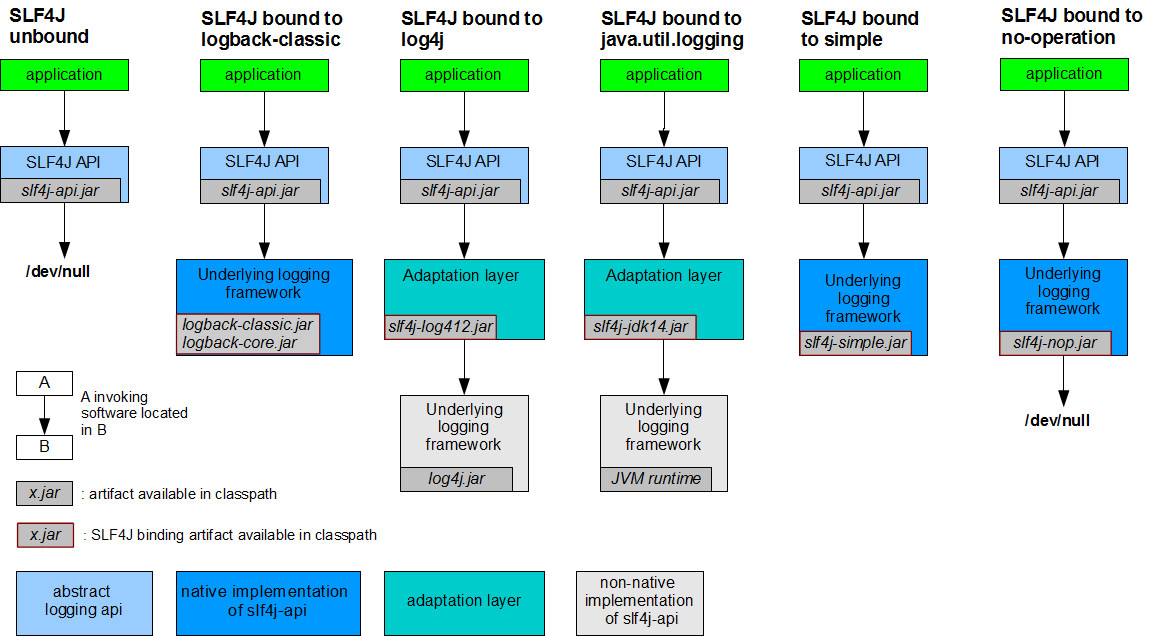
\includegraphics[width=\textwidth]{slf4jBindings.png}
		\end{center}
	\end{frame}

	\begin{frame}[fragile]
		\frametitle{Пример}
		\begin{footnotesize}
			\begin{minted}{java}
import org.slf4j.Logger;
import org.slf4j.LoggerFactory;

public class Wombat {
  private final Logger logger = LoggerFactory.getLogger(Wombat.class);
  private Integer t;
  private Integer oldT;

  public void setTemperature(Integer temperature) {
    oldT = t;
    t = temperature;

    logger.debug("Temperature set to {}. Old temperature was {}.", t, oldT);

    if(temperature.intValue() > 50) {
      logger.info("Temperature has risen above 50 degrees.");
    }
  }
} 
			\end{minted}
		\end{footnotesize}
\end{frame}

	\begin{frame}
		\frametitle{SLF4J}
		\begin{itemize}
			\item Умеет многое из того, что умеют ``настоящие'' библиотеки, так что можно просто выводить в лог, не задумываясь об API
			\begin{itemize}
				\item Формирование строк через \{\}
				\item Маркеры
			\end{itemize}
			\item Чтобы всё работало, надо подключить:
			\begin{itemize}
				\item slf4j-api --- обязательно, и одно из:
				\item slf4j-simple --- бэкенд ``из коробки'', умеет выводить в System.err
				\item log4j-slf4j-impl --- для использования Log4J в качестве бэкенда
			\end{itemize}
			\item Не забываем конфигурационный файл Log4J, если используем как бэкенд его
		\end{itemize}
	\end{frame}

\end{document}
